\section{Preliminaries}
\label{sec:preli}
% motivation
\begin{figure}
  \centering
  {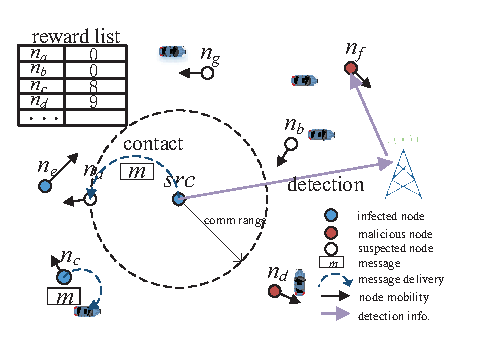
\includegraphics[width=0.47\textwidth]{fig/sketch.eps}}
     \caption{Reward and Detection of the selfish nodes in OppNets.}
     \label{fig:sketch}
\end{figure}
The source node $src$ needs to disseminate its message $m$
to vehicles or pedestrians,
where the lifetime of $m$ is $T$.
There are $N$ relay nodes that can receive $m$ and broadcast $m$,
which is shown in Fig.~\ref{fig:sketch}.
Thus the potential coverage area of $m$ 
is broadened by the opportunistic network.
$src$ usually reward the relay node 
$n_{i}$ $(1 \le i \le N)$ for its collaboration,
where the reward can be quantifies as the message carrying time.
However, $n_{i}$ may discard $m$ immediately after the contact
to earn the reward without carrying $m$,
which is the selfish behavior.
For example, when the contact between $src$ and $n_{i}$ occurs,
$m$ is replicated $n_{i}$ at time $\tau_{0}$, which is recorded by $src$.
If $n_{i}$ carries $m$ until the lifetime $T$,
the reward, which is proportional to $T-\tau_{0}$,
will be offered to $n_{i}$ for its contribution.
But if $n_{i}$ discards $m$ at time $\tau_{1}$,
$\tau_{0} < \tau_{1} < T$,
a part of reward, $T-\tau_{1}$, is wasted
because $src$ can not obtain $\tau_{1}$.

To decrease the wasted reward,
$src$ can conduct the selfish node detection,
whose process are as follows.
%Assume the size of message $m$ is $L$ bytes,
1) $src$ first randomly select the target relay node $n_{i}$ 
and the message segment $L$.
2) $src$ send the query of $L$'s checksum to $n_{i}$ 
via the wireless communication, e.g., the cellular network.
3) If the check of $n_{i}$ failed,
$n_{i}$ would not receive the reward from the detection time.
Note that the minimum cycle of a detection process is $T_{m}$,
which is constrained by the computation of checksum and 
the communication of querying.
%check the checksum of $m$'s specific part,
%which is store in the randomly selected relay node $n_{i}$.
%If the check failed,
%$n_{i}$ will be identified as the selfish node
%and can not receive the reward.
In this paper, we will propose the optimal selfish node detection strategy
to achieve the tradeoff between the detection cost 
and the wasted reward by selfish behaviors.

%1.Poisson process of contacts
%2.Poisson process of being selfish
$R(t)$ denotes the expected number of the relay nodes,
which have not contacted $src$ before time $t$.
$I(t)$ denotes the expected number of infected relay nodes,
which still carry $m$ at time $t$.
$D(t)$ denotes the expected number of selfish relay nodes,
which have discarded $m$ but are not known by $src$ at time $t$.
Similar to \cite{TCSS2018ControlM} and \cite{CC2007PerfAnaly},
the contacts between $src$ and every relay node
are assumed to occur according to the Poisson process,
where the contact rate is $\lambda$.
The total number of relay nodes is $N$.
So $N=R(t)+I(t)+D(t)$, $\forall t$, $0 \le t \le T$.
We assume the rate of change
from state I to state D is a constant value $\rho$.
The detection rate is $U(t)$,
$0 \le U(t) \le U_{m}$.
which can be controlled by $src$.
For example, if the minimum detection cycle $T_{m}$ is $0.5$ seconds,
the maximum detection rate is that $U_{m} = \frac{1}{T_{m}} = 2$
times per second.
%To simplify the denotations,
%we use $R(t)$, $I(t)$ and $D(t)$ to
%replace $E(R(t))$, $E(I(t))$ and $E(D(t))$,
%respectively.
Then the main objective of our work is to
to solve the following problem,
\begin{small}
\begin{equation}
\label{eq:obj}
\begin{aligned}
Min: J &= \int_{0}^{T} (1-\alpha) D(t) + \alpha U(t) dt ,
\end{aligned}
\end{equation}
\end{small}
where $\alpha$ is the constant weight, $0 \le \alpha \le 1$.
This objective will minimize the reward,
which is paid to the selfish nodes in state $D$
and the detection cost.
Additionally, the total paid reward is,
\begin{small}
\begin{equation}
\label{eq:reward}
\begin{aligned}
P &= \int_{0}^{T} \beta ( I(t) + D(t) )dt,
\end{aligned}
\end{equation}
\end{small}
where $\beta$ is the reward paid for 
a node's contribution in a second.
In order to realize our proposed detection,
we also should ensure $P$ is limited in OppNet.
